\chapter{Исходный код реализации процедур предобучения и редуцирования}
\label{app:a}

\begin{lstlisting}[style=PythonStyle]
import torch
import torch.nn as nn
from common_types import InitTypes

class UnifiedClassifier(nn.Module):
    def __init__(self, layers_config):
        super().__init__()
        self.layers = nn.ModuleList()
        self.a_functions = []
        self.layers_config = layers_config["architecture"]
        layer_index = 0
        for layer in self.layers_config:
            if len(layer[0]) == 2:
                new_layer = nn.Linear(*layer[0])
            if len(layer[0]) == 3:
                new_layer = nn.Conv2d(*layer[0])
            self.layers.append(new_layer)
            self.a_functions.append(layer[1][-1])
            layer_index += 1

    def forward(self, x):
        for layer, afunc, layer_config in zip(self.layers, self.a_functions, self.layers_config):
            x = afunc(layer(x))
            if len(layer_config) == 3:
                post_processing_actions = layer_config[2]
                for action in post_processing_actions:
                    x = action(x)
        return x

class RBM(nn.Module):
    def __init__(self, n_vis, n_hid, a_func, init_type, without_sampling):
        super(RBM, self).__init__()
        if init_type == InitTypes.Kaiming:
            W = torch.empty(n_vis, n_hid)
            v = torch.empty(1, n_vis)
            h = torch.empty(1, n_hid)
            torch.nn.init.kaiming_normal_(W, mode='fan_out', nonlinearity="relu")
            torch.nn.init.kaiming_normal_(v, mode='fan_out', nonlinearity="relu")
            torch.nn.init.kaiming_normal_(h, mode='fan_out', nonlinearity="relu")
            self.W = nn.Parameter(W)
            self.v = nn.Parameter(v)
            self.h = nn.Parameter(h)
        elif init_type == InitTypes.SimpleNormal:
            self.W = nn.Parameter(0.1 * torch.randn(n_vis, n_hid))
            self.v = nn.Parameter(torch.zeros(1, n_vis))
            self.h = nn.Parameter(-1 * torch.ones(1, n_hid))
        elif init_type == InitTypes.SimpleUniform:
            self.W = nn.Parameter(0.02 * torch.rand(n_vis, n_hid)-0.01)
            self.v = nn.Parameter(0.02 * torch.rand(1, n_vis)-0.01)
            self.h = nn.Parameter(0.02 * torch.rand(1, n_hid)-0.01)
        self.a_func = a_func
        self.without_sampling = without_sampling

    def visible_to_hidden(self, v):
        weighted_sum = torch.mm(v, self.W) + self.h
        output = self.a_func[1](weighted_sum)
        return output, weighted_sum

    def hidden_to_visible(self, h):
        weighted_sum = torch.mm(h, self.W.t()) + self.v
        output = self.a_func[0](weighted_sum)
        return output, weighted_sum

    def forward(self, v0):
        h0, h0_ws = self.visible_to_hidden(v0)
        if self.without_sampling:
            h_sampled = h0
        else:
            if self.a_func[1] == torch.sigmoid:
                h_sampled = 1. * (h0 > torch.rand(h0.shape))
            elif self.a_func[1] == torch.relu:
                h0_std = torch.std(h0, dim=0, unbiased=False)
                h_sampled = h0 + torch.normal(0, h0_std)
            else:
                h_sampled = h0
        v1, v1_ws = self.hidden_to_visible(h_sampled)
        h1, h1_ws = self.visible_to_hidden(v1)
        return v0, v1, v1_ws, h0, h0_ws, h1, h1_ws

    def __str__(self) -> str:
        return "vis: " + str(self.v.shape) + \
               "hid: " + str(self.h.shape)
               
class CRBM(nn.Module):
    def __init__(self, n_vis_channels, n_hid_channels, kernel_size, a_func, init_type, without_sampling):
        super(CRBM, self).__init__()
        if init_type == InitTypes.Kaiming:
            W = torch.empty(n_hid_channels, n_vis_channels, kernel_size, kernel_size)
            torch.nn.init.kaiming_normal_(W, nonlinearity="relu")
            self.W = nn.Parameter(W)
        elif init_type == InitTypes.SimpleNormal:
            self.W = nn.Parameter(0.01 * torch.randn(n_hid_channels, n_vis_channels, kernel_size, kernel_size))
        elif init_type == InitTypes.SimpleUniform:
            self.W = nn.Parameter(0.02 * torch.randn(n_hid_channels, n_vis_channels, kernel_size, kernel_size) - 0.01)
        self.a_func = a_func
        self.without_sampling = without_sampling

    def visible_to_hidden(self, v):
        weighted_sum = torch.convolution(v, self.W, None, stride=[1,1], padding=[0,0], dilation=[1,1], transposed=False, output_padding=[0,0], groups=1)
        output = self.a_func[1](weighted_sum)
        return output, weighted_sum

    def hidden_to_visible(self, h):
        weighted_sum = torch.conv_transpose2d(h, self.W, None, stride=[1, 1], padding=[0, 0], output_padding=[0, 0], groups=1,
                               dilation=[1, 1])
        output = self.a_func[0](weighted_sum)
        return output, weighted_sum

    def forward(self, v0):
        h0, h0_ws = self.visible_to_hidden(v0)
        if self.without_sampling:
            h_sampled = h0
        else:
            if self.a_func[1] == torch.sigmoid:
                h_sampled = 1. * (h0 > torch.rand(h0.shape))
            elif self.a_func[1] == torch.relu:
                h0_std = torch.std(h0, dim=0, unbiased=False)
                h_sampled = h0 + torch.normal(0, h0_std)
            else:
                h_sampled = h0
        v1, v1_ws = self.hidden_to_visible(h_sampled)
        h1, h1_ws = self.visible_to_hidden(v1)
        return v0, v1, v1_ws, h0, h0_ws, h1, h1_ws

    def __str__(self) -> str:
        return "vis: " + str(self.v.shape) + \
               "hid: " + str(self.h.shape)
               
import torch
from torch import nn
import utilities as utl
import config
from models import RBM, CRBM

class RBMStack:
    def __init__(self, layers_config, device, init_type, without_sampling):
        self.rbm_stack = []
        self.layers = layers_config["architecture"]
        self.input_dim = layers_config["input_dim"]
        self.device = device
        for i in range(0, len(self.layers) - 1):
            layer_params = self.layers[i][0]
            layer_activation_function = self.layers[i][1]
            rbm_constructor = RBM if len(layer_params) == 2 else CRBM
            rbm = rbm_constructor(*layer_params, layer_activation_function, init_type, without_sampling)
            self.rbm_stack.append(rbm.to(self.device))

    def _prepare_train_set(self, train_set, batch_size, input_dim, layer_index=0):
        batches_count = len(train_set) / batch_size
        if isinstance(input_dim, tuple):
            resulted_array = torch.zeros((train_set.shape[0], *input_dim))
        else:
            resulted_array = torch.zeros((train_set.shape[0], input_dim))
        i = 0
        while i < batches_count:
            _slice = slice(i * batch_size, (i + 1) * batch_size)
            inputs = train_set[_slice]
            if layer_index == 0:
                resulted_array[_slice] = inputs
            else:
                inputs = inputs.to(self.device)
                v0, v1, v1_ws, h0, h0_ws, h1, h1_ws = self.rbm_stack[layer_index - 1](inputs)
                resulted_array[_slice] = h0
            i += 1
        if len(self.layers[layer_index - 1]) == 3:
            post_processing_actions = self.layers[layer_index - 1][2]
            for action in post_processing_actions:
                if not isinstance(action, torch.nn.Dropout):
                    resulted_array = action(resulted_array)
        return resulted_array

    def train(self, train_set, pretrain_type):
        layers_losses = {}
        train_set = self._prepare_train_set(train_set, config.pretraining_batch_size, self.input_dim)
        batches_count = len(train_set) / config.pretraining_batch_size
        layer_index = 0
        with torch.no_grad():
            for rbm, layer in zip(self.rbm_stack, self.layers):
                output_shape = utl.train_rbm_with_custom_dataset(
                    train_set, self.device, rbm, pretrain_type, batches_count)
                layer_index += 1
                train_set = self._prepare_train_set(train_set, config.pretraining_batch_size, output_shape[1:],
                                                    layer_index)
        return layers_losses

    def torch_model_init_from_weights(self, torch_model):
        with torch.no_grad():
            for i in range(0, len(torch_model.layers) - 1):
                if len(torch_model.layers_config[i][0]) == 2:
                    torch_model.layers[i].weight.data = self.rbm_stack[i].W.T
                    torch_model.layers[i].bias.data = torch.reshape(self.rbm_stack[i].h, (len(self.rbm_stack[i].h[0]),))
                if len(torch_model.layers_config[i][0]) == 3:
                    torch_model.layers[i].weight.data = self.rbm_stack[i].W

    def do_reduction(self, layers_config):
        with torch.no_grad():
            for i in range(0, len(self.layers) - 1):
                mask = torch.abs(self.rbm_stack[i].W) > config.reduction_param
                self.rbm_stack[i].W *= mask.double()
            condition = None
            for i in range(0, len(self.layers) - 1):
                if condition is not None:
                    self.rbm_stack[i].W = nn.Parameter(self.rbm_stack[i].W[condition])
                condition = torch.abs(self.rbm_stack[i].W).sum(dim=0) != 0
                self.rbm_stack[i].W = nn.Parameter(self.rbm_stack[i].W[:, condition])
                self.rbm_stack[i].h = nn.Parameter(self.rbm_stack[i].h[:, condition])
                layers_config["architecture"][i][0] = tuple(self.rbm_stack[i].W.shape)
            previous_neurons_count = layers_config["architecture"][len(self.layers)-2][0][1]
            end_layer_neurons_count = layers_config["architecture"][len(self.layers)-1][0][1]
            layers_config["architecture"][len(self.layers)-1][0] = (previous_neurons_count, end_layer_neurons_count)
            
import random
import config
import torchvision.datasets as datasets
import torch
from rbm_stack import RBMStack
from models import UnifiedClassifier
from torch import nn
import torch.optim as optim
import data_config
import torch.nn.functional as F
from common_types import PretrainingType, DatasetType, Statistics
from models import RBM

def get_random_seeds(count):
    seeds = []
    for i in range(0, count):
        seeds.append(random.randint(0, config.max_random_seed))
    return seeds

def get_dataset_constructor(dataset_type: DatasetType):
    dataset_selector = {
        DatasetType.MNIST: datasets.MNIST,
        DatasetType.CIFAR10: datasets.CIFAR10,
        DatasetType.CIFAR100: datasets.CIFAR100
    }
    return dataset_selector[dataset_type]

def train_rbm_with_custom_dataset(train_set, device, rbm, pretrain_type, batches_count):
    train_func = train_rbm if isinstance(rbm, RBM) else train_crbm
    losses, output_shape = train_func(rbm, device, batches_count, train_set, pretrain_type)
    return output_shape

def train_rbm(rbm, device, batches_count, train_set, pretrain_type):
    delta_weights = torch.zeros(rbm.W.shape).to(device)
    delta_v_thresholds = torch.zeros(rbm.v.shape).to(device)
    delta_h_thresholds = torch.zeros(rbm.h.shape).to(device)
    losses = []
    act_func = rbm.a_func
    for epoch in range(config.pretraining_epochs):
        loss = 0.
        i = 0
        momentum = config.momentum_beg if epoch < config.momentum_change_epoch else config.momentum_end
        while i < batches_count:
            inputs = train_set[i * config.pretraining_batch_size:(i + 1) * config.pretraining_batch_size].to(device)
            v0, v1, v1_ws, h0, h0_ws, h1, h1_ws = rbm(inputs)
            if pretrain_type == PretrainingType.RBMClassic:
                der_v, der_h = 1, 1
                rate = config.pretraining_rate
            elif pretrain_type == PretrainingType.REBA:
                der_v = (act_func[0](v1_ws + 0.00001) - act_func[0](v1_ws - 0.00001)) / 0.00002
                der_h = (act_func[1](h1_ws + 0.00001) - act_func[1](h1_ws - 0.00001)) / 0.00002
                rate = config.pretraining_rate_reba
            if config.with_adaptive_rate:
                b_h = h0 * ((v1 * v0).sum() + 1) - h1 * (1 + (v1 * v1).sum())
                b_v = v0 * (1 + (h0 * h0).sum()) - v1 * (1 + (h0 * h1).sum())
                rate = (((v0-v1) * b_v).sum() + ((h0-h1) * b_h).sum()) / ((b_h*b_h).sum() + (b_v*b_v).sum())
            part_v = (v1 - v0) * der_v
            part_h = (h1 - h0) * der_h
            delta_weights = delta_weights * momentum + rate / config.pretraining_batch_size * (
                    torch.mm(part_v.T, h0) + torch.mm(v1.T, part_h))
            delta_v_thresholds = delta_v_thresholds * momentum + rate / config.pretraining_batch_size * part_v.sum(0)
            delta_h_thresholds = delta_h_thresholds * momentum + rate / config.pretraining_batch_size * part_h.sum(0)
            rbm.W -= delta_weights
            rbm.v -= delta_v_thresholds
            rbm.h -= delta_h_thresholds
            part_loss = ((v1 - v0) ** 2).sum()
            loss += part_loss.item()
            i += 1
        losses.append(loss)
    return losses, h0.shape

def train_crbm(rbm, device, batches_count, train_set, pretrain_type):
    delta_weights = torch.zeros(rbm.W.shape).to(device)
    losses = []
    act_func = rbm.a_func
    for epoch in range(config.pretraining_epochs):
        loss = 0.0
        i = 0
        momentum = config.momentum_beg if epoch < config.momentum_change_epoch else config.momentum_end
        while i < batches_count:
            inputs = train_set[i * config.pretraining_batch_size:(i + 1) * config.pretraining_batch_size].to(device)
            v0, v1, v1_ws, h0, h0_ws, h1, h1_ws = rbm(inputs)
            if pretrain_type == PretrainingType.RBMClassic:
                der_v, der_h = 1, 1
                rate = config.pretraining_rate
            if pretrain_type == PretrainingType.REBA:
                der_v = (act_func[0](v1_ws+0.00001) - act_func[0](v1_ws-0.00001)) / 0.00002
                der_h = (act_func[1](h1_ws+0.00001) - act_func[1](h1_ws-0.00001)) / 0.00002
                rate = config.pretraining_rate_reba
            part_v = (v1 - v0) * der_v
            part_h = (h1 - h0) * der_h
            first_convolution_part = torch.convolution(
                torch.permute(part_v, (1, 0, 2, 3)),
                torch.permute(h0, (1, 0, 2, 3)), None, stride=[1,1], padding=[0,0], dilation=[1,1], transposed=False, output_padding=[0,0], groups=1)
            second_convolution_part = torch.convolution(
                torch.permute(v1, (1, 0, 2, 3)),
                torch.permute(part_h, (1, 0, 2, 3)), None, stride=[1,1], padding=[0,0], dilation=[1,1], transposed=False, output_padding=[0,0], groups=1)
            common_conv_expr = first_convolution_part + second_convolution_part

            delta_weights = delta_weights * momentum + rate / config.pretraining_batch_size * torch.permute(common_conv_expr, (1, 0, 2, 3))
            rbm.W -= delta_weights
            loss += ((v1 - v0) ** 2).sum()
            i += 1
        losses.append(loss.item())
    return losses, h0.shape

def train_torch_model(model, train_loader, test_loader, optimizer, criterion, device):
    best_total_accuracy = 0
    losses = []
    for epoch in range(config.finetuning_epochs):
        running_loss = 0.0
        for i, data in enumerate(train_loader, 0):
            inputs, labels = data[0].to(device), data[1].to(device)
            optimizer.zero_grad()
            outputs = model(inputs)
            loss = criterion(outputs, labels)
            loss.backward()
            optimizer.step()
            running_loss += loss.item()
        if epoch % config.test_every_epochs == 0:
            current_accuracy = test_torch_model(model, test_loader, device)
            if current_accuracy > best_total_accuracy:
                best_total_accuracy = current_accuracy
        losses.append(running_loss)
    return best_total_accuracy, losses

def test_torch_model(model, test_loader, device):
    correct_answers = 0
    with torch.no_grad():
        for data in test_loader:
            images, labels = data[0].to(device), data[1].to(device)
            outputs = model(images)
            _, predictions = torch.max(outputs, 1)
            correct_answers += (predictions == labels).sum()
    return 100 * float(correct_answers) / len(test_loader.dataset)

def run_experiment(layers_config, pretrain_type, meta_data, device, init_type, without_sampling):
    rbm_stack = RBMStack(layers_config, device, init_type, without_sampling)
    layers_losses = None
    train_loader = meta_data[2]
    train_set = data_config.get_tensor_dataset_from_loader(train_loader)
    if pretrain_type != PretrainingType.Without:
        layers_losses = rbm_stack.train(train_set, pretrain_type)
        if config.with_reduction:
            rbm_stack.do_reduction(layers_config)
    classifier = UnifiedClassifier(layers_config).to(device)
    rbm_stack.torch_model_init_from_weights(classifier)
    criterion = nn.CrossEntropyLoss(reduction="sum")
    optimizer = optim.SGD(classifier.parameters(), lr=config.finetune_rate, momentum=config.finetuning_momentum, weight_decay=1e-6)
    test_loader = meta_data[3]
    best_total_acc, losses = train_torch_model(classifier, train_loader, test_loader, optimizer, criterion, device)
    return Statistics.get_train_statistics(layers_losses, best_total_acc), losses
\end{lstlisting}

\chapter{Документы об использовании результатов диссертационной работы}
\label{app:b}

\begin{figure}[ht]
	\centering
	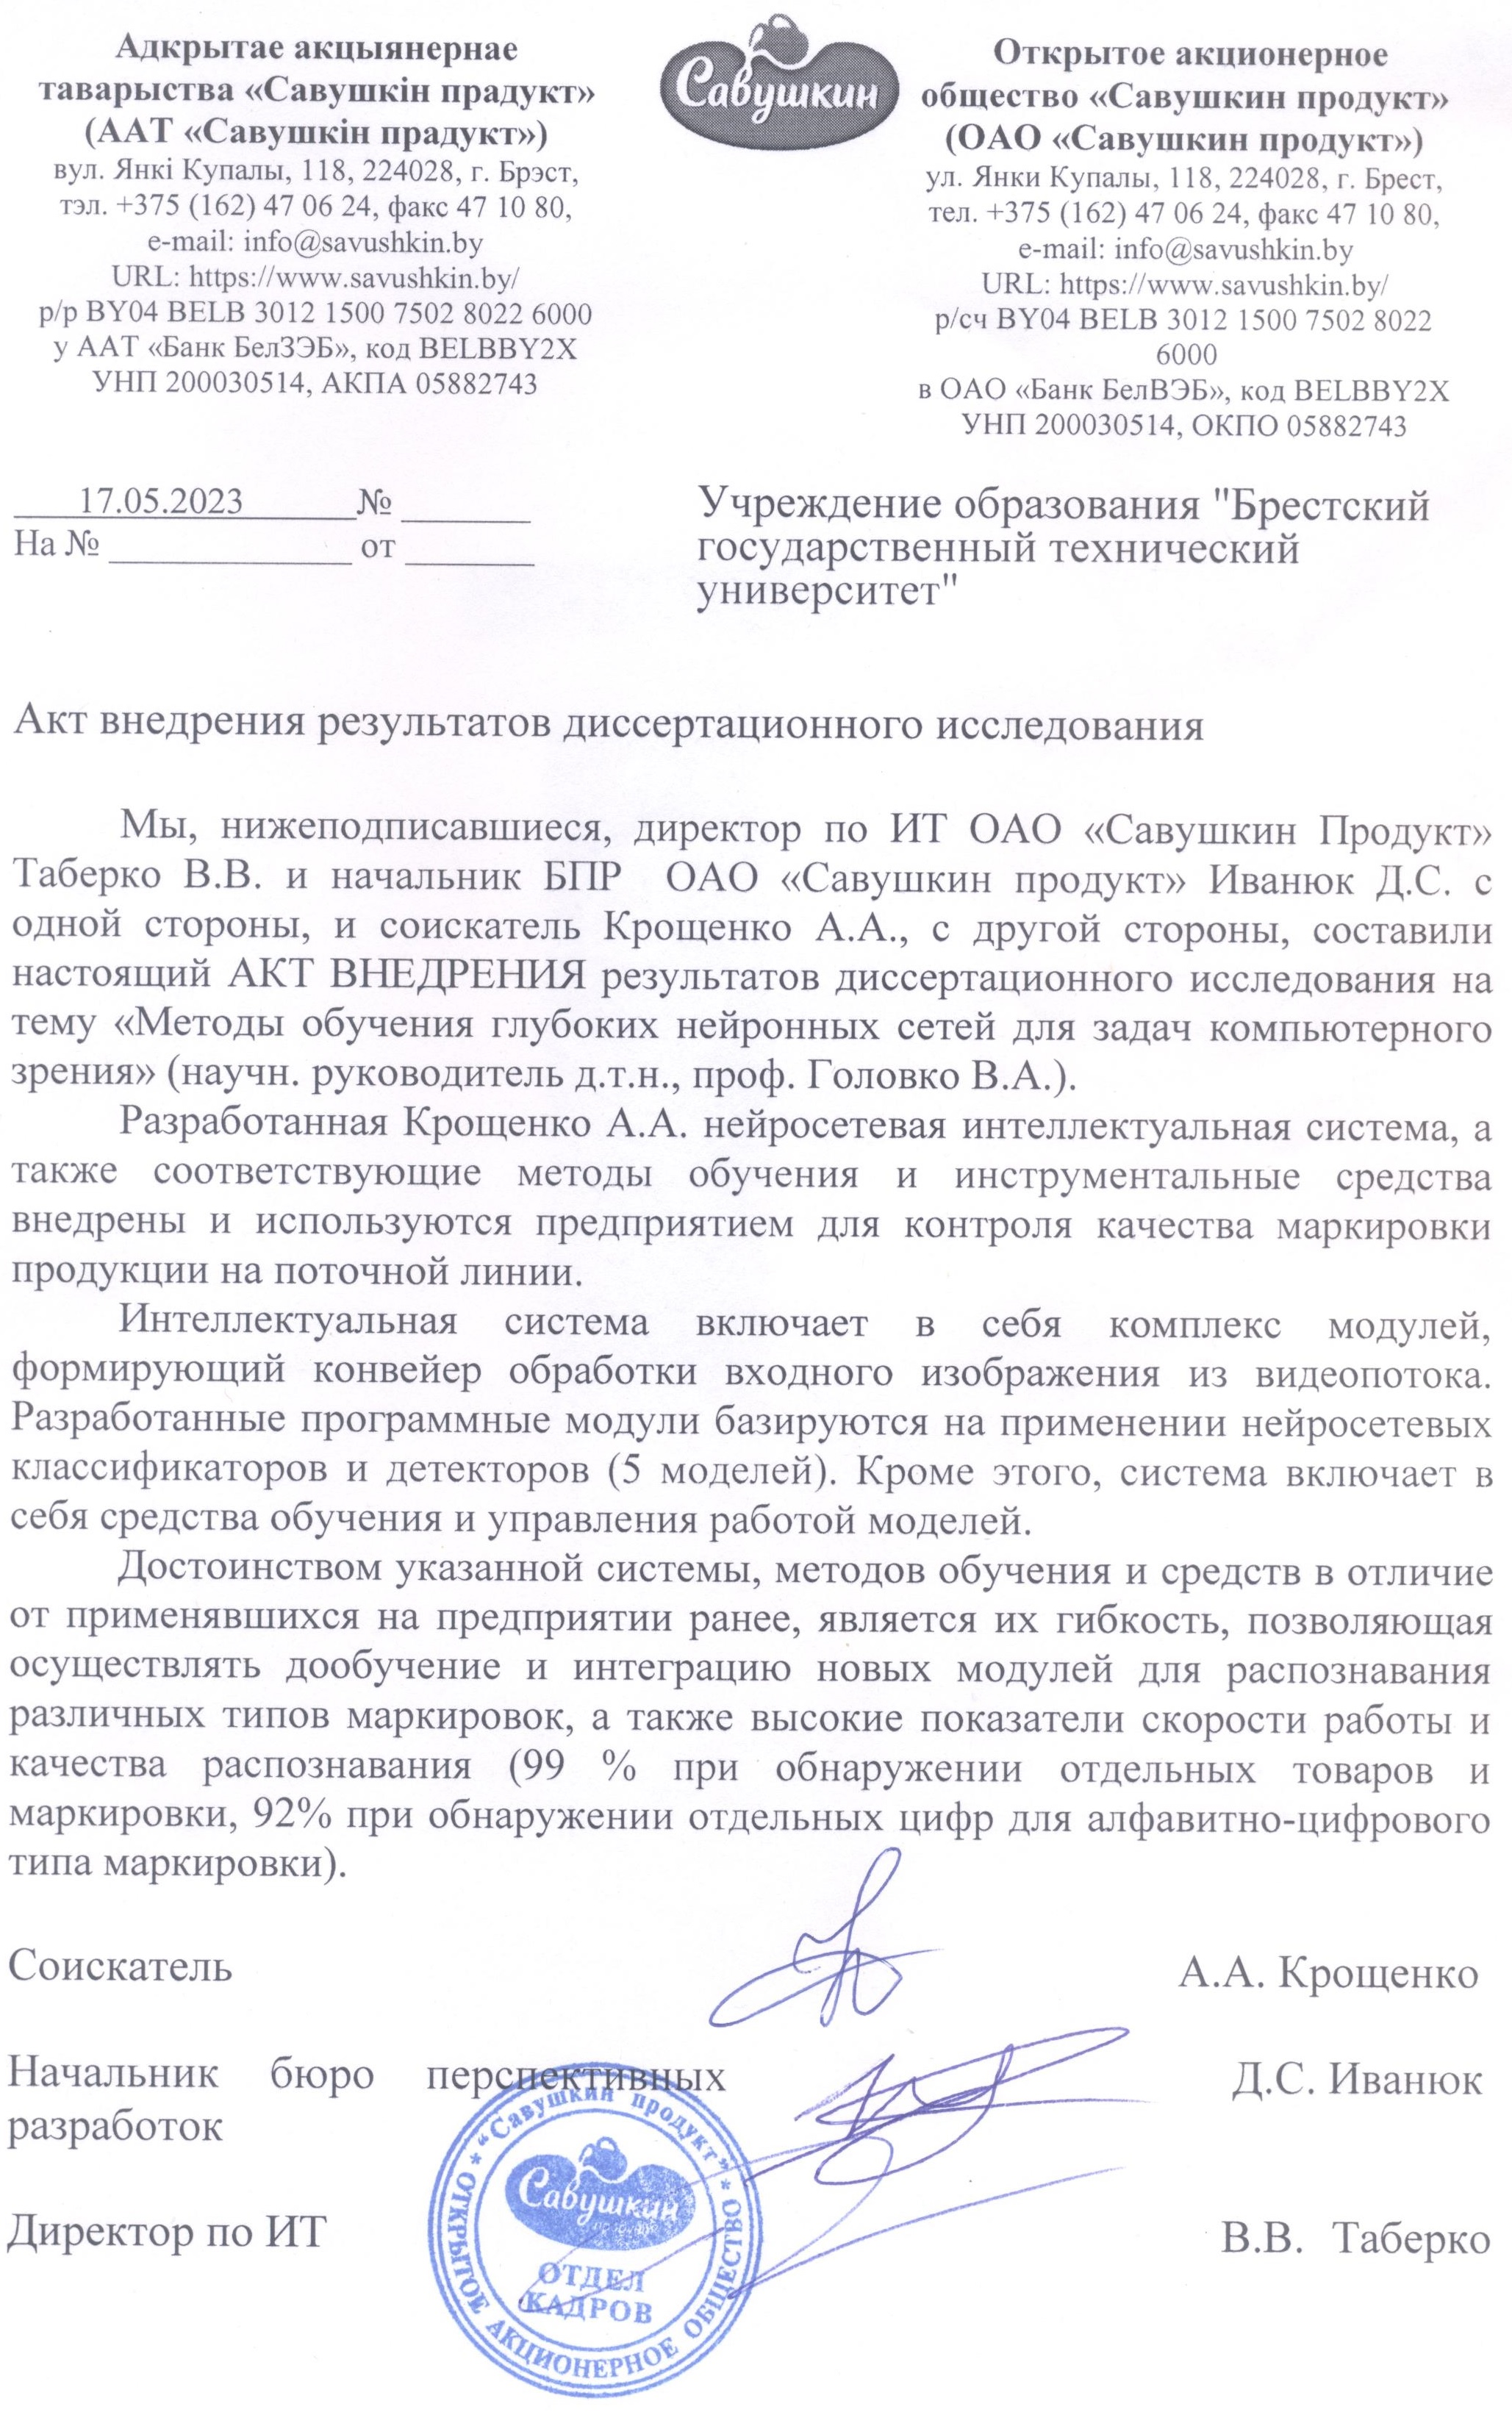
\includegraphics[height=20cm]{man-source/images/appendix/appendixActs/act_Savushkin.jpg}
\end{figure}

\begin{figure}[ht]
	\centering
	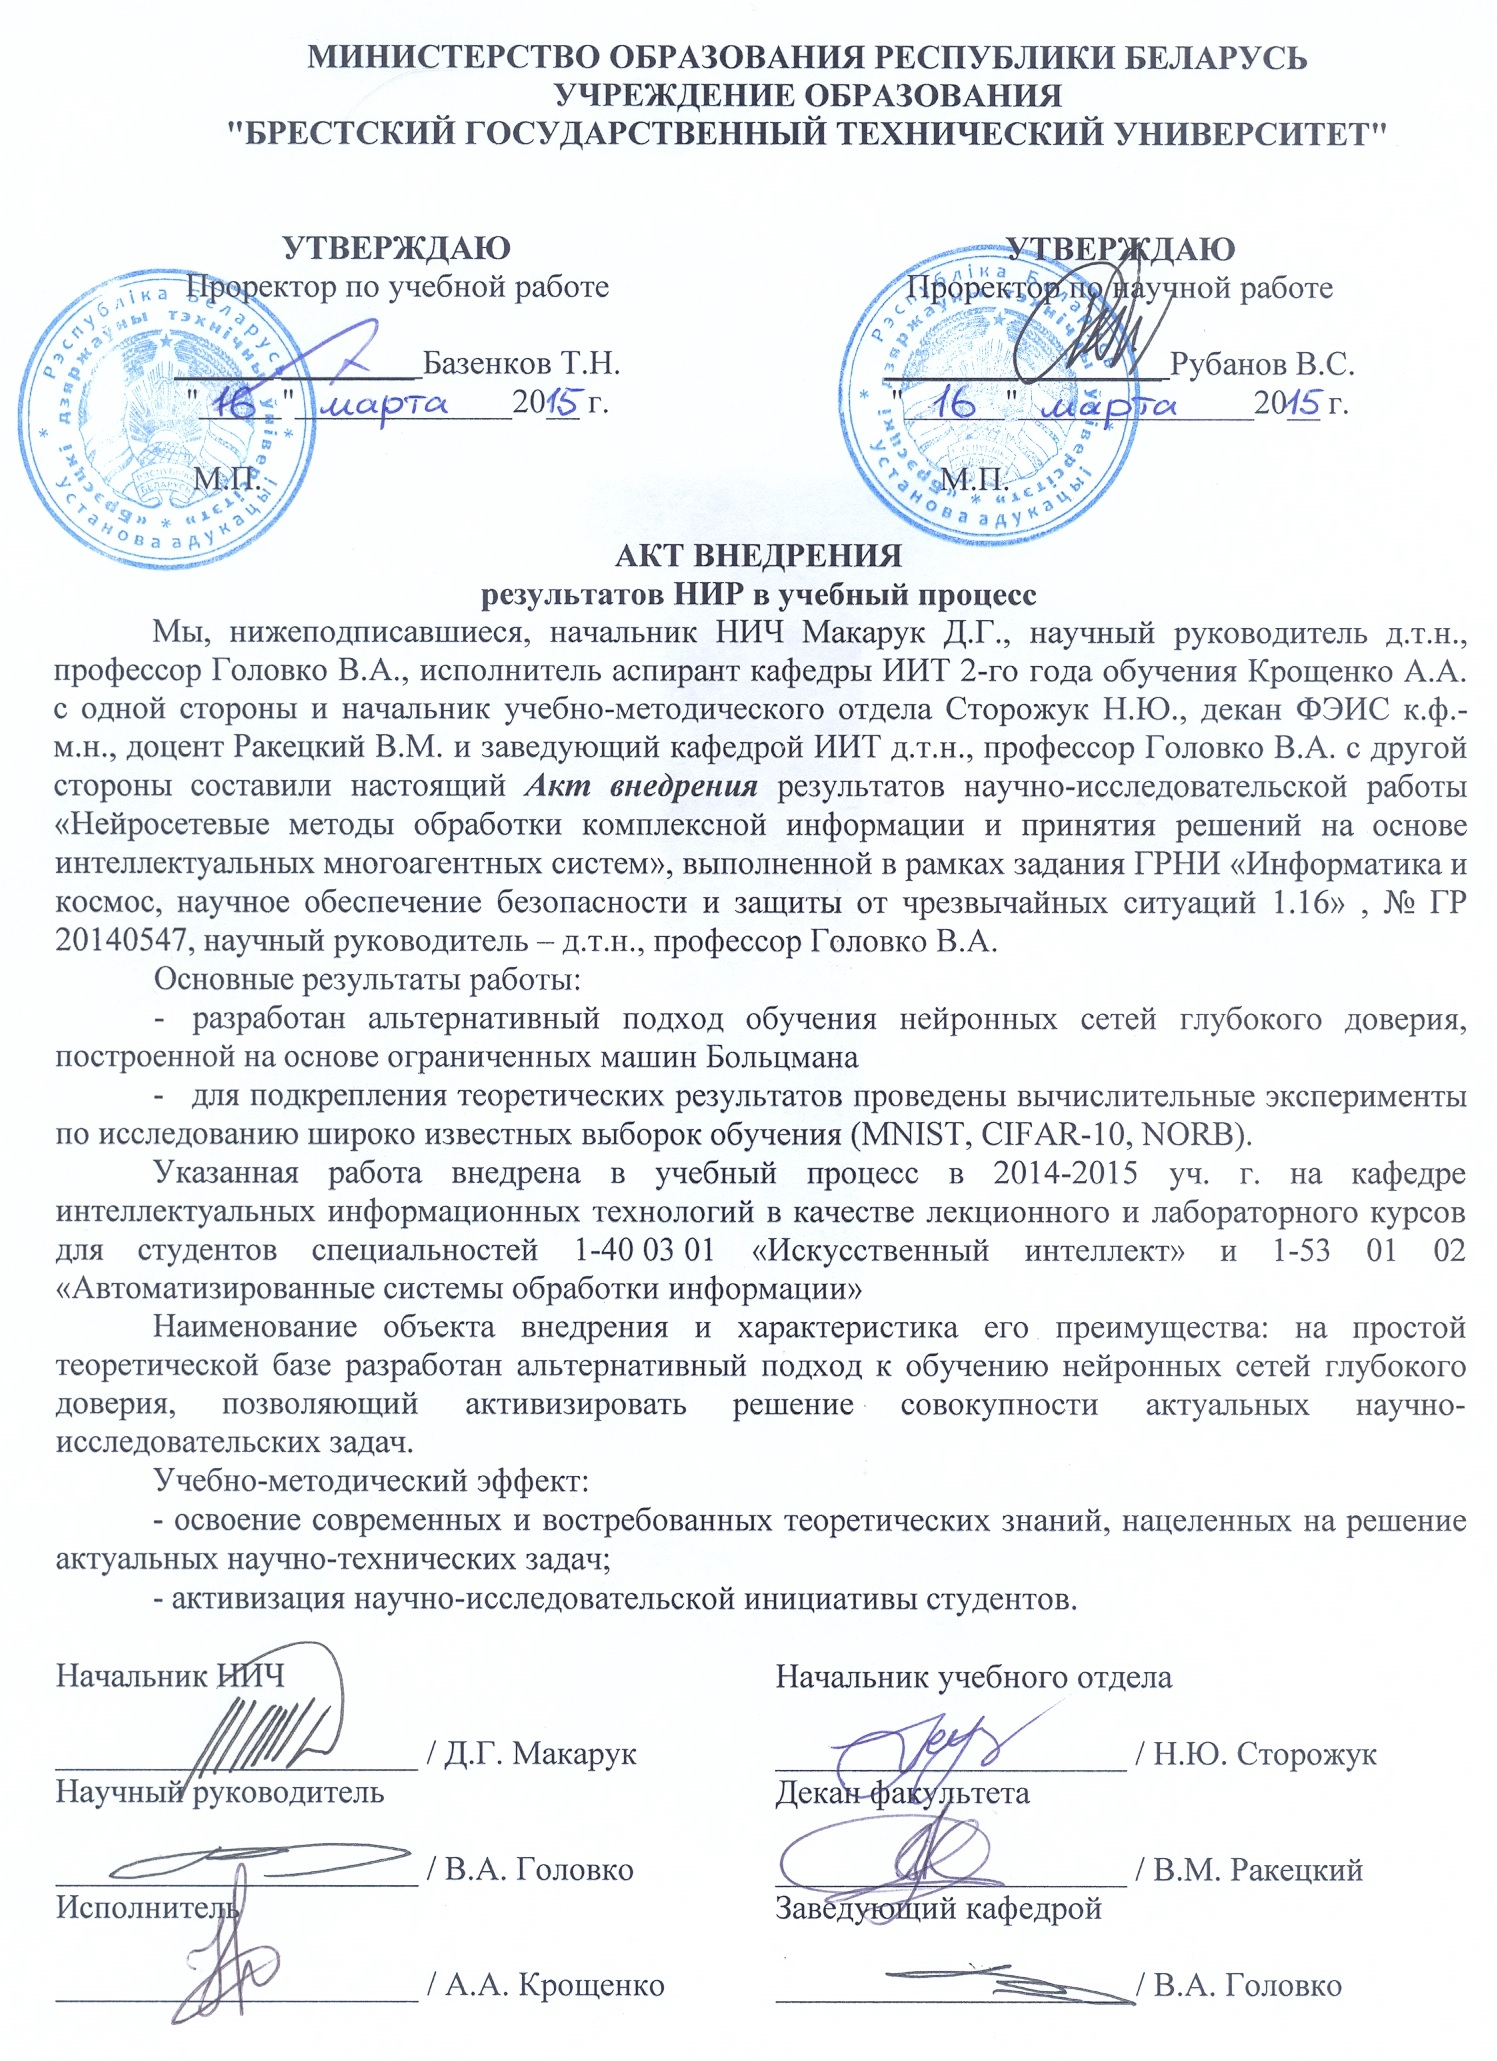
\includegraphics[height=23cm]{man-source/images/appendix/appendixActs/act_BSTU.jpg}
\end{figure}

\begin{figure}[ht]
	\centering
	
\includegraphics[width=17cm]{man-source/images/appendix/appendixActs/act_ISS-2.jpg}
\end{figure}
